%KELOMPOK 2 Pemasukan
%\begin{itemize}
%\item Imron Sumadireja (1164076)
%\item Jesron Marudut Hatuan (1164077)
%\item Lusia Violita Aprilian (1164080)
%\item Mhd. Zulfikar Akram Nst. (1164081)
%\end{itemize}

\section{Pengertian HTTP}
Protokol HTTP atau Hypertext Transfer Protocol merupakan sebuah protokol untuk meminta dan menjawab antara client dengan server. HTTP juga merupakan protokol jaringan lapisan aplikasi yang digunakan untuk sistem informasi terdistribusi, kolaboratif, dan menggunakan hypermedia. Misalnya pada aplikasi mobile dan Dropbox Service HTTP digunakan  sebagai protokol yang dapat mendistribusikan animasi gambar dan suara yang bersumber dari Dropbox Service.

\subsection{HTTP Protokol Untuk Streaming}
HTTP protokol digunakan dalam streaming karena protokol ini sangat mudah untuk diakses dimanapun. HTTP protokol ini menyediakan movie dari standart web server dengan nama lain `pseudo streaming' atau `progressive download' dikenal juga dengan fast start. Pada saat kita mendownload sebuah video dan filenya sudah di download tetapi bisa di play pada saat sebelum download selesai. Terlihat seperti true streaming. HTTP bisa memiliki data rate yang lebih tinggi, sehingga bisa memiliki kualitas yang lebih tinggi, bahkan untuk file yang telah di download bisa di play berulang - ulang. HTTP juga bisa untuk streaming semua jenis data quicktime\cite{putra2010analisis}.

\subsection{Kemampuan protokol HTTP}
Sebagai sebuah protokol jaringan aplikasi yang digunakan untuk sistem informasi terdistribusi, Hypertext Transfer Protokol (HTTP) mempunyai kemampuan sebagai berikut ini;
1. Hypertext Transfer Protokol (HTTP) mampu mengirim tipe data yang komplit sama halnya dengan satu pesan yang memakai satu format untuk MIME mail internet. Sebab itu sebuah Website dapat melebihi hypertext ke hypertmedia dan website server dapat melayani client dengan informasi informasi yang berupa teks, suara, video dan grafik yang diintergrasikan menggunakan dokumen HTML.
2. Hypertext Transfer Protocol dapat memfasilitasi komunikasi antar protokol lain yang mengunakan gateway yang berbeda dengan client HTTP. Dari skema penamaan URL mengidentifikasikan bahwa tidak lokasi saja tetapi protokol yang dibutuhkan untuk menerima sumber dayanya\cite{lusiana2009sistem}.

\subsection{cara menggunakan HTTP melalui TLS}
Secara konseptual, HTTP / TLS sangat sederhana, Cukup gunakan HTTP melalui TLS seperti menggunakan HTTP melalui TCP. Agen yang bertindak sebagai klien HTTP yang juga harus bertindak sebagai klien TLS. Hal ini harus terkoneksi ke server pada port yang sesuai dan kemudian mengirim Klien TLS. Ketika hubungan TLS telah selesai. Klien kemudian dapat memulai permintaan HTTP pertama. Semua data HTTP harus dikirim sebagai "data aplikasi" TLS. HTTP berjalan normal, termasuk koneksi yang dipertahankan, harus diikuti\cite{rescorla2000http}.

\section{HTTP versi 2}
HTTP versi 2 adalah versi berikutnya dari HTTP dan didasarkan pada Google SPDY, yang dirancang untuk mempercepat loading halaman web dan pengalaman browsing. HTTP versi 2 adalah standar baru dan akan mengambil alih protokol HTTP yang saat ini digunakan oleh sebagian besar situs di internet. HTTP versi 2 ini merupakan protokol yang lebih modern, dimana http versi 2 dapat meningkatkan kecepatan browsing web dengan menggunakan cara-cara terbaru. HTTP versi 2 lebih cepat dari HTTP dalam hal transfer rate, hal ini dipengarui oleh salah satunya, yaitu server push. Adanya server push membantu mengurangi waktu tunggu yang dialami oleh browser\cite{engku2016analisis}.

\subsection{Tujuan HTTP versi 2}
HTTP versi 2 merupakan sebuah protokol web versi terbaru yang baru saja diresmikan standarnya oleh IETF. Tujuan utamanya dibuat HTTP versi 2 adalah untuk memperbaiki kelemahan yang ada pada HTTP versi 1.1 salah satu kelemahannya yakni ketika browser meminta halaman, server akan mengirimkan dokumen HTML, kemudian perlu menunggu browser untuk mengurai dokumen HTML untuk memunculkan request untuk semua aset yang tertanam, sebelum server dapat mengirim JavaScript, gambar dan CSS. Teknologi server push pada HTTP versi 2 memungkinkan server untuk menghindari perputaran ini dengan cara `mendorong' aset-aset baru dari server ke klien\cite{engku2016analisis}.

\section{Sistem Komunikasi Langsung Multimedia Yang Terhubung Dengan HTTP Protocol}
Sistem komunikasi langsung multimedia yang terhubung dengan Protokol HTTP terdiri dari program aplikasi dan Server Web, di mana program aplikasi diinstal menjadi sejumlah komputer pribadi klien (PC), berada di dalamnya PC sedemikian rupa sehingga mereka ditampilkan selama berjam-jam di PCS menempati sebagian Ruang pada tampilan PC, dan terhubung setiap saat dengan server Web melalui HTTP; Web server memiliki antarmuka CGI dan terhubung ke masing-masing PCS melalui sirkuit komunikasi untuk mengeksekusi Program dan aplikasi komunikasi HTTP, dan masing-masing klien dapat mentransfer (chat) surat elektronik dengan satu sama lain pseudo-real time Via Internet dan / atau Intranet menggunakan program aplikasi\cite{nishizawa2005multimedia}.

\section{Versi HTTP}
Dalam skema penomoran, HTTP menggunakan skema "<Major>.<Minor>" untuk menunjukkan versi versi dari setiap prtotokol. Kebijakan dibuatnya versi protokol untuk memungkinkan pengirim untuk memilih format pesan dan kapasitas dalam memahami setiap komunikasi HTTP lebih lanjut, dari pada fitur-fitur yang diperoleh melalui komunikasi. Dan tidak hanya perbedaan yang dibuat ke nomor untuk setiap versi agar penambahan komponen-komponen pesan yang tidak mempengaruhi sifat dari komunikasi tersebut\cite{berners1996hypertext}.

\section{HTTP Message}
Http Messages adalah rangkaian blok data yang dikirim antar aplikasi HTTP. Blok data diawali dengan teks yang berisi meta information. Teks ini menggambarkan konten pesan dari HTTP message. Setiap HTTP message berisi tentang request dari client atau response dari server. HTTP message terbagi menjadi 3 bagian, yaitu: start line, headers, dan body\cite{hartono2013desain}.

\subsection{3 Bagian HTTP Message}
Start Line merupakan bagian pertama dari HTTP message yang memberikan gambaran data yang dikirim. Header merupakan bagian HTTPmessage yang berfungsi untuk memberikan informasi atribut data. Sedangkan bagian Body merupakan bagian HTTP message yang berisi pesan yang inign dikirim. Pada penggunaannya terdapat perbedaan formmat penulisan HTTP message yang dikirimkan dari client ke server (http request) dengan HTTP message yang dikirimkan dari server ke client (http response)\cite{hartono2013desain}.

\section{Kompatibilitas HTTP dengan Proxy, Firewalls, dan NAT}
Salah satu alasan mengapa penggunaan HTTP adalah kemampuannya untuk lulus melalui proksi, firewall, atau penerjemah alamat jaringan (NAT). Satu konsekuensi yang tidak menguntungkan dari firewall dan NAT adalah yang mereka dibuat lebih sulit untuk menyebarkan aplikasi Internet baru, dengan meminta eksplisit izin (atau bahkan peningkatan perangkat lunak firewall atau NAT) pada akomodasi setiap protokol baru. Keberadaan firewall dan NAT menciptakan insentif yang kuat untuk perancang protokol untuk lapisan baru aplikasi di atas protokol yang ada, termasuk HTTP. Namun, jika firewall situs mencegah penggunaan protokol yang tidak dikenal, ini agaknya merupakan keputusan kebijakan yang sadar dari pihak administrator firewall. Sementara itu dapat diperdebatkan bahwa kebijakan tersebut nilai terbatas dalam meningkatkan keamanan, di samping itu nomor port terkenal sangat berguna untuk berbagai tujuan, dan kelebihan nomor port mengikis utilitas ini. Mencoba untuk menghindari kebijakan keamanan situs tidak dapat diterima pembenaran untuk melakukannya. Akan berguna untuk menetapkan pedoman untuk "firewall-friendly" protokol, untuk memudahkan firewall yang ada agar kompatibel dengan protokol baru
\cite{moore2002use}.

\section{Konsep Web Client dan Web Server}

\begin{figure}[ht]
\centerline{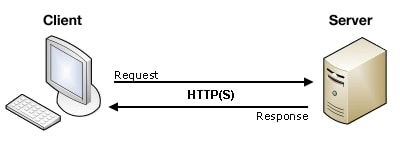
\includegraphics[width=1\textwidth]{figures/2http.jpg}}
\caption{Client Server}
\label{2http}
\end{figure}

Pada gambar \ref{2http} dijelaskan bahwa setiap web content berada pada web server. Web server berkomunikasi menggunakan HTTP sebagai protokol, maka sering disebut sebagai HTTP server. Proses pengiriman data dimulai dari HTTP client yang mengirimkan HTTP request ke server. HTTP request tersebut akan diterima dan diolah oleh server, kemudian server akan mengirimkan kembali HTTP response pada client. HTTP client dan HTTP server merupakan komponen yang membentuk World Wide Web (WWW).

